\section{RHUL New Edwards Depositions\label{sec:edwards500}}
  \newcommand{\imedwardsFiveHundred}{\hyperref[sec:edwards500]{\textit{\textbf{\underline{Edwards 500}}}}}
  
  Machine is located in clean room, used for depositing \textbf{gold, nickel, titanium aluminium.} \red{Very important to get the valve system in the right order.}
  \subsection{Switching machine on}
   The machine is initially in the off state. First we need to get the pumps of the machine up and running.
   \begin{enumerate}
   	\item On the black `button board' \cmd{turn the dial on the top middle sector from 0 to 1} to turn the machine on.
   	\item The green screen directly to the right should light up. \texttt{Select `MANUAL MODE'} out of the possible options.
   	\item \texttt{Scroll to ``RELAY-INPUTS'' \ra Press ``YES''}. \red{Check that everything is \iitem{OFF}!}
   	\item \cmd{Go to \iitem{1 ROT PUMP} option \ra press \iitem{ON}.} This turns on the rotary pump.
   	\item \cmd{Go to \iitem{3 BACKING V.} option \ra press \iitem{ON}.} Now the turbo molecular pump is being pumped.
   	\item \cmd{Go behind the machine, and check that the black box is receiving power.} Red light below \iitem{POWER IN} should be on.
   	\item Open up the chamber directly under the main chamber. At the very back is th turbo molecular pump switch - \red{A red switch.} \cmd{Flick it \red{down} to start the turbo molecular pump. If it starts flashing red, turn it on and off again.}
   \end{enumerate}

 \begin{figure}[htbp]
 	\centering
 	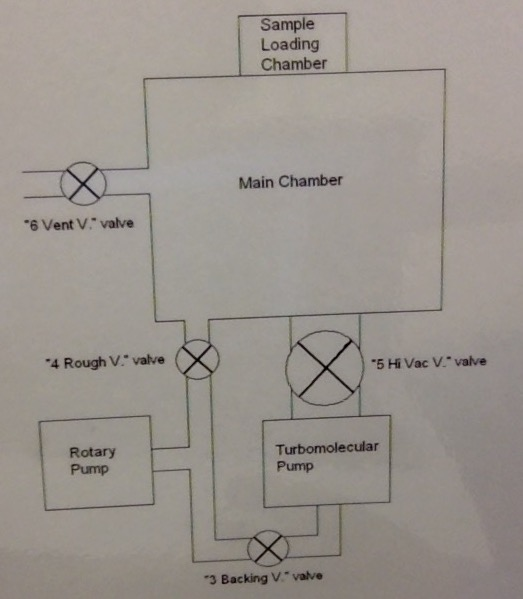
\includegraphics[height=10cm]{dia}
 \end{figure}
 \subsection{Loading}
  To load, we need to vent the chamber and open the door.
  \red{Prior to loading double check that \cmd{\mi{4 ROUGH V.} \mi{5 HIGH VAC V.}} are off!}
 \begin{enumerate}
  \item \cmd{Go to \mi{6 VENT V} options \ra Will read \mi{OFF} \ra Press \mi{YES} \ra Will go to \mi{ON}.}
  \item \cmd{Press \ino \ra Will read \imonitor \ra Press \iyes to enter menu.} Chamber pressure displayed.
  \item When pressure gauge read $ 10^3 $MB, \cmd{Press \ino.}
  \item \cmd{Go to \irelayinputs \ra Press \iyes.}
  \item \cmd{Go to \ivent option \ra Reads \ion \ra Press \iyes \ra Now reads \ioff.} \red{THIS IS SO WE DONT FORGET TO CLOSE THE VALVE AFTERWARDS AND SCREW UP THE TURBO PUMP.}
  \item Chamber can now be opened and loaded. 
  \item Check the material level by \cmd{Go to \mi{TURRET CONTROL PANEL} \ra Select material \ra Press the \mi{0/1 BUTTON} \ra The motor switches on.\ra Remember to switch the \mi{0/1 BUTTON} off.}
 \end{enumerate}
  
 \subsection{Pumping the main Chamber}
  Once the sample is loaded
  \begin{enumerate}
  	\item \cmd{Go to \irelayinputs \ra Press \iyes.}
  	\item \cmd{Go to \ivent option \ra Check if reads \ioff (If not press \iyes to set to to \ioff.)} This is to prevent the venting of the main chamber.
  	\item \cmd{Go to \ibacking option \ra Press \iyes \ra Now reads \ioff}. This is to isolate the turbo pump from the main chamber.
  	\item \cmd{Go to \irough option \ra Press \iyes \ra Now reads \ion.} This causes the rotary pump to pump the main chamber.
  	\item \cmd{Press \ino Now reads \imonitor \ra Press \iyes \ra Chamber pressure displayed. Wait until 0.5MB reached.}
  	\item \cmd{Press \ino \ra Go to \irelayinputs \ra Press \iyes.}
  	\item \cmd{Go to \irough \ra Press \iyes\ra Now reads \ioff. \red{Wait 10-15 seconds.}} This prepares the rotary pump for helping the turbo one.
  	\item \cmd{Go to \ibacking option \ra Press \iyes \ra Now reads \ion.} We now pump the turbo pump with the normal one.
  	\item \cmd{Go to \ihighvac option \ra Press \iyes \ra Now reads \ion.} The turbo pump is now pumping the main chamber.
  	\item \cmd{Press \ino \ra Go to \imonitor \ra Press \iyes \ra \red{Check pressure is decreasing.}}
  	\item \cmd{Press \ino \ra Go to \ipenning menu \ra Press \iyes.}
  	\item \cmd{Press \iyes \ra Now reads \iheadon.} This turns on the sensitive pressure meter. If it doesn't turn on, repeat until it does.
  	\item \cmd{Press \ino \ra Go to \imonitor \ra Press \iyes \ra \red{Leave to pump until $ 5*10^{-5} $MBar}.}
  \end{enumerate}


 \subsection{Crucible deposition}
  \begin{enumerate}
  	\item \textbf{\mi{TURRET CONTROL}} is where one selects the material to deposition. \cmd{Turn the dial to the desired position \ra Press the \mi{0/1 Button} to activate the motor and make it turn. Remember to turn it off afterwards though. \mi{On}} means the motor it running, \mi{o$ \backslash $l} means it is not moving. A yellow light indicates the turret position;
  	\item \textbf{\mi{SWEEP CONTROL}} is where one adjusts the beam. The raw settings are
  	\begin{itemize}
  		\item X = z waveform, \red{15 frequency}, middle amplitude;
  		\item Y = sinusoid waveform, \red{8 frequency}, middle amplitude.
  	\end{itemize}
  	\item \textbf{\mi{SOURCE CONTROL}} is where one sets the accelerating voltage and the current for crucibnle deposition.
  	\item \red{\textbf{\mi{SOURCE SHUTTER}} \ra \cmd{Press middle button} to set it into remote mode. This way whenever the required thickness is reached (via LabView or manual procedure) the shutter will close automatically.} 
  	\red{If you want to control the shutter manually, \cmd{Do NOT press the middle button.} Instead be prepared to \cmd{Press SS1 button} (left hand side) to open and close to the shutter manually.}
  		\item Activate the \textbf{\mi{FTM7}} where one sets the deposition parameters. \cmd{Click on \mi{DATA} button to change between the menus.} \red{Alternatively run \mi{FTM7\_set\_parameters.vi} from LabView to set the material and thickness! }
  	\begin{itemize}
  		\item \textbf{Rate} gives the current deposition rate;
  		\item \textbf{Layer} is what material is being deposited. There is a sheet in the lab saying what layer corresponds to what material. E.g. for Au it it layer 4. \cmd{\red{Set to the required material!}};
  		\item \textbf{Density and z-Value (acoutstic impedance)} are set depending on the layer chosen. They depend on the material used - \red{\cmd{set to the required material.}};
  		\item \red{\textbf{Terminate} is were we set the thickness after which to close the shutter. \cmd{\red{Set the required thickness.}};}
  		\item \textbf{Tooling} sets the ratio of the distances of the quartz thickness crystal and the samples from the crucible. \red{Set to 1.0}
  		\item \textbf{xTal} selects which of the 2 crystal we are going to use. \red{By default set to 1 - \textbf{the crystal in the right hand side of the chamber}} 
  		\item \textbf{Usage} indicates how much the crystal has been used out of 100\%.
  	\end{itemize}
 \end{enumerate}

 With this basic setup, one can proceed via two routes to perform the deposition.

 \subsubsection{Gun deposition (i.e. we do it manually)}
	\begin{enumerate} 
	\item \cmd{Set the deposition parameters on \mi{FTM7}.}
	\item \cmd{Go to \mi{SWEEP CONTROL} panel turn the dial \red{0$ \rightarrow $ 1.}}
	\item \cmd{Go to \mi{SOURCE CONTROL} panel \ra Press \mi{ON/OFF}.}
	\item \cmd{Press \mi{GUN} button to allow local control \ra Voltage should jump to \red{5kV}.}
	\item \cmd{Slowly ramp up the current 0mA\ra20mA\ra40mA\ra\red{No more than 120mA!} and monitor the deposition rate on the \mi{FTM7} panel.}
	\item When a steady reading is produced (0.10nm/s) \cmd{Press \mi{RUN} on the \mi{FTM7} panel to open the shutter}. Deposition proceeds, and the shutter will close automatically once the \red{set thickness is reached}. Shutter can be out in manual mode by `unpressing' the \mi{REMOTE SHUTTER} button and operating the \mi{SS1} button.
	\item \red{Make sure that there are no explosions in the crucible. Lower current if required.}
	\item Once done, shutter will close. \cmd{Slowly ramp the current down to 0 \ra Turn off \mi{GUN} \ra Turn off \mi{SOURCE CONTROL} \ra Turn off \mi{SWEEP CONTROL}.}
  \end{enumerate}
  
   \subsubsection{Local/Remote deposition (usingLabView\label{sssec:depositLab})}
    LabView is when the deposition is controlled from the LabView program.
    
    \begin{enumerate}
    	\item \cmd{Log into \mi{Administrator} with empty password.}
    	\item \cmd{Load \cmd{Evaporation Control Program.}}
    	\item \cmd{Choose material \ra choose thickness \ra choose rate. Do not worry about the turret option - then turret you have set manually is the one that will be used in the deposition.} \red{\cmd{Run program \ra press start \ra wait until shutter lights turns on and off \ra stop program} to set parameters on \mi{FTM7}.}
    	\item \cmd{Go to \mi{SOURCE CONTROL} panel \ra Press \mi{ON/OFF} \ra Voltage should jump to \red{5kV}.}
    	\item \cmd{Press \mi{LOCAL/REMOTE} button to allow LabView to control the current.}
    	\item \cmd{RUN the program.} The rate will be reached (current 10-100mA) \ra Shutter opened \ra Set thickness deposited \ra Shutter closed \ra current ramped down. \red{If an error occurs, manually lower the current by slowly lowering current value in \mi{Electron Gun.vi} to 0mA.}
    	\item Turn off \mi{REMOVE/LOCAL} \ra Turn off \mi{SOURCE CONTROL} \ra Turn off \mi{SWEEP CONTROL}.
    \end{enumerate}
 \subsection{Boat or spiral deposition}
  \red{There is no shutter for this deposition! We do not touch the source control panel, but use the one with HT, LT and big 0-11 dial}
  
  \begin{itemize}
  	\item \cmd{Set the deposition parameters on \mi{FTM7}.}
  	\item \cmd{\red{\textbf{Ensure that the middle source shutter button is NOT pressed}} \ra press \mi{Run} on \mi{FTM7}} to begin accumulation from 0;
  	\item The front and back voltage supplies are chosen \cmd{using LT selectors \mi{front} and \mi{back} respectivily};
  	\item \cmd{Choose \mi{LT} on the LT-O-HT dial} to activate the voltage supply;
  	\item \cmd{\mi{Reset} and begin ramping up the current};
  	\item \cmd{Once \mi{FTM7} shows the required thickness \ra \red{press \mi{trip}} and turn the dial to LT-0-HT}
  \end{itemize}
 
 \subsection{Venting the main chamber}
  Once the deposition is performed \red{wait 5 minutes} before taking the sample out.
  \begin{enumerate}
  	\item \cmd{Press \ino \ra \imonitor \ra Go to \ipenning menu \ra Press \iyes to enter.}
  	\item \cmd{\iheadon will be displayed \ra Press \iyes \ra Now reads \iheadoff.} We need to turn off the sensitive gauge to avoid damaging it.
  	\item \cmd{Press \ino \ra Go to \irelayinputs \ra Press \iyes.}
  	\item \cmd{Go to \ihighvac option \ra Will read \ion \ra Press \iyes \ra Will go to \ioff.} Thus we stop pumping the main chamber. \red{Wait 40 seconds.}
  	\item \cmd{Go to \ivent option \ra Will read \ioff \ra Press \iyes \ra Will go to \ion.} The chamber begins to vent.
  	\item \cmd{Press \ino \ra Will read \imonitor \ra Press \iyes to enter menu.} Chamber pressure displayed.
  	\item When pressure gauge read $ 10^3 $MB, \cmd{Press \ino.}
  	\item \cmd{Go to \irelayinputs \ra Press \iyes.}
  	\item \cmd{Go to \ivent option \ra Reads \ion \ra Press \iyes \ra Now reads \ioff.} \red{THIS IS SO WE DONT FORGET TO CLOSE THE VALVE AFTERWARDS AND SCREW UP THE TURBO PUMP.}
  	\item Chamber can now be opened and loaded. 
  \end{enumerate}


  {\LARGE Before leaving, remember to rough pump the main chamber and \red{turn on the turbo molecular pump to pump the main chamber! If you don't put the backing on, it will de pressurise over time and damage the pump}.
  }
  
 \newpage
 